\section*{Sanctions as a Network Process \& the Importance of Reciprocity}
\label{neteffects}

One contribution of this study is to argue and demonstrate why sanctions processes should be considered in a network context. To do so, we provide an example. Figure \ref{fig:spaghetti} presents the entire sanction-year network for the year 1984.  Nodes represent states and the directed edges denote the sender and receiver of sanctions. This figure is complex, showing that each yearly network contains important information about state behavior, whereby numerous states are involved in multiple sanction cases during this individual year.  IR scholars typically treat each dyad as independent, despite that a singular actor, such as the USA, likely exist within multiple dyads. The appearance of multiple actors in multiple rows of the data violates assumptions of independence. Theoretically, however, this also means that scholars are unable to include analysis of second-order dependencies such as reciprocity into their studies. While studies of international relations tend to recognize the interdependent nature of state behavior in the theoretical sense, they often fail to uphold this theoretical intuition in empirical analysis. Early attempts are noteworthy,\footnote{\cite{keohane1989reciprocity,goldstein1991reciprocity}} and more recent work has continued to address this concern,\footnote{\cite{mitchell2001,cranmer2014reciprocity}} yet studies on sanction compliance have not incorporated these insights. 

\begin{figure}[ht]
  \centering
  \begin{tabular}{c}
	  \includegraphics[width=1\textwidth]{84net-crop} \\
	  \includegraphics[width=0.45\textwidth]{MapLegend}
  \end{tabular}
  \caption{Here we show the sanction network in 1984, nodes are colored by geographic coordinates of countries. Data for sanction cases comes from \citet{morgan2009threat}.}
  \label{fig:spaghetti}
\end{figure}
\FloatBarrier


%CD: S, can you add a bit more here? maybe walk us through more about the network? not sure but it feels a bit brief.


\subsection*{Theoretical Expectations of Reciprocity and State Behavior}
Assuming that sanctions can thus be considered through a network lens, we can then move forward to better incorporate concepts such as reciprocity into our analysis. Given the wide range of literature on reciprocity in IR, we argue that it is necessary to consider how reciprocity plays a role in determining why, and when, sanctions end.

 In studies of social and economic behavior, direct reciprocity--the notion that actors learn to ``respond in kind" to one another--is argued to be an essential component of behavior.\footnote{For example, see \cite{bolton:1998, charness:2002, charness:2004, cox:2007, cox:2004}.} The idea that individuals, or collectives, observe previously cooperative (or conflictual) behavior from others, and include this information into their own decision-making process, is a concept given great value to determine strategic outcomes. For example, reciprocity is shown to influence interactions across diverse settings including tax compliance \citep{smith:1990}, wage selection \citep{campbell:1997}, and strike breaking \citep{brett:1998}. Reciprocity is also shown to play a critical role in the development of interethnic attitudes whereby groups tend to reflect the attitudes that other groups hold toward them \citep{berry:1979}. 

Intuition about reciprocity's effect on the behavior of individuals also extends to aggregate analysis. International Relations and foreign policy scholars have expressed a long standing interest in how reciprocity influences the evolution of cooperative and conflictual interactions among states \citep{richardson1960, keohane1989reciprocity}. \cite{rajmaira:1990} argue that reciprocity determines long-term foreign policy behavior among superpowers via norms creation. The authors importantly point out that reciprocity is a non-static mechanism which changes over time. They show that while mutual reactivity between superpowers is often weak, high peaks in reciprocity create long-lasting and influential norms of behavior between countries. In other realms of international politics, reciprocity plays a key role in formulating expectations of state behavior. \cite{ward1981} even argued that reciprocity is a ``golden rule" of politics between nations.  Osiel similarly notes, ``It is an empirical datum that people tend to respond to others with an implicit policy of like for like and that this facilitates cooperation between them. This elementary fact has profound implications for the effective design of law and institutions.'' \cite[p. 19]{osiel:2009}. Reciprocity has long been recognized by IR scholars as an important mechanism for the enforcement of agreements and instantiation of cooperation. 

While reciprocity receives little attention in sanctions research, much of the literature instead focuses on how specific types of relationships between senders and targets--such as alliances and trade ties--expedite sanction resolution. The core mechanisms driving sanction outcomes are thus characterized in terms of a cost-benefit analysis, ignoring the plausible role that reciprocity plays in driving state behavior. Underlying the relational dimensions explored in the literature is the concise argument that there are some set of countries from whom the sending of sanctions are more consequential, and will thus be complied to more quickly, than others. However, by ignoring reciprocity the extant analyses of these linkages disregards the rich history of interactions between two countries. We argue that reciprocal interactions provide a fundamental reflection of the strategic environment that shapes state's compliance behavior. More specifically, we posit that reciprocity influences sanction outcomes through informing future expectations of behavior between states. 

Overtime, previous reciprocal interactions inform a target state's decision to comply more swiftly, or to delay compliance to show resolve rather than cooperation. Our basic intuition is to expect that when a target state has a richer history of reciprocal compliance with sender states, they will more swiftly comply with the senders' demands. The primary hypothesis of this study, is thus that \textit{reciprocity creates an underlying level of expected behavior which influences patterns of compliance among target states.}

Importantly, our claim does not demand that reciprocity always work in some inherently ``good'' or ``bad'' way, but instead can work to prolong or shorten sanctions depending on which kind of past reciprocal behavior has occurred. This concept thus requires that we specify which forms of reciprocity should matter in the case of sanctions. We argue that reciprocity influences sanction outcomes through two forms: \textit{compliance reciprocity} and \textit{sanction reciprocity}. 

%CD: more on reciprocity in this context here


We first outline the compliance reciprocity measure. This measure represents a target states' cumulative history of compliance with a particular sender relative to all others in the network. Our measure of compliance reciprocity allows us to capture whether those who have a history of cooperative behavior with each other also tend to have more cooperative behavior in the future. In a duration context, states who receive sanctions from those with whom they have a history of reciprocal compliance are likely to comply sooner, than they would with lower states to whom they have not had positive reciprocal interactions. 

Notably, this measure is distinct from a simple counter of past instances of compliance with another state. Such a measure would completely ignore the fact that each state's actions are conditional on all other interactions between states. For example, if state $i$ complies often to state $j$, is state $i$ also more likely to comply with all other partner states? Or, relative to all other interactions, does state $i$ comply more frequently and uniquely with state $j$? The latter idea is the one explicated within our  concept of compliance reciprocity. Thus, reciprocity tells us information about the behavior between country $i$ and $j$ over time, relative to how country $i$ interacts with all other partners over time. 

%CD: dotchart or some plot of COMPLIANCE reciprocity over time goes HERE


We extend this intuition to our second key concept, \textit{sanction reciprocity}. Following the same idea as compliance reciprocity, this is a measure of how often a target state has received sanctions from the senders of any given sanction case -- relative to all other sanction interactions of states. The intuition behind this measure is to capture the concept of creating expectations of resolve: states who have been sanctioned multiple times by a sender state are likely to build up a willingness of resistance and not cooperation. This suggests that states receiving sanctions from those with whom they have been sanctioned before are likely to more slowly comply with those states. 

The basic insight is that states whom continually respond to sanctions by sending sanctions of their own are signaling more conflictual rather than cooperative behavior over time. This strategic environment is a dominating factor for the initiation of sanction compliance. Thus, in a world of changing information and strategic incentives, a country will not continue to repetitively comply with a partner state simply out of perceived strategic ties. Countries require continuous signals to build trust and cooperation over time and to maintain a shared understanding of strategic importance to one another.


%CD: dotchard or some plot of sanction reciprocity here



%NOW we turn to how to measure, and conclude:
To operationalize our measure of reciprocity, we turn to the Social Relations Model developed by \citet{kenny1994interpersonal} and (author removed). To illustrate, consider the matrix $X_{ij}$ below, in which we have six actors in a round robin (dyadic) format. These data are represented by the matrix below, which has a value for each of the thirty interactions, with the main diagonal remaining empty:

\singlespacing
\[
\left[
\begin{array}{cccccc}
 & X_{12}  & X_{13}  & X_{14} & X_{15} & X_{16} \\
X_{21}  &  & X_{23}  & X_{24} & X_{25} & X_{26} \\
X_{31}  & X_{32}  &    & X_{34} & X_{35} & X_{36} \\
X_{41}  & X_{42}  & X_{43}  &  & X_{45} & X_{46} \\
X_{51}  & X_{52}  & X_{53}  & X_{54} &   & X_{56} \\
X_{61}  & X_{62}  & X_{63}  & X_{64} & X_{65} &   \\
\end{array}
\right]
\]

\doublespacing
First, we begin with calculating the row column and total sums:

\begin{itemize}
	\item The totals for each \emph{ row} are denoted $X_{i \cdot}$ where $i$ is the row number, i.e.,
	~\\
	$X_{i \cdot} = \sum_{j=1}^{J} X_{ij}$;
	\item For each column the totals are denoted
	 $X_{\cdot i}$ where $i$ is the \emph{column} number; and 
	 \item The total over all rows and columns is given by $X_{\cdot \cdot} = \sum_i \sum_j X_{i,j}$.
 \end{itemize}
 
Given these quantities, one can calculate individual effects for a variety of concepts, such as the actor, partner, and unique dyadic effects, (as well as the variances attributed to each of these effects). The unique dyadic effects, or the reciprocal interactions between two countries within one pair, are calculated accounting for the general behavior of each country within the pair. Or, in other words, this measure captures how likely country $i$ is to comply with country $j$; and the likelihood that country $j$ is to comply with country $i$ is calculated relative to how often country $i$ tends to comply with all of the other countries, as well as how likely country $j$ is to comply with all others. 

 \begin{itemize}
	 \item The actor effect for observation $i$ is the total of $i$'s row mean and column mean, minus the overall mean.  The means are just the sums, corrected for degrees of freedom, yielding an average row effect:\\
	 $\hat{a}_i = \frac{(n-1)^2}{n(n-2)} X_{i \cdot} + \frac{(n-1)}{n(n-2)} X_{\cdot i} -  \frac{n-1}{n-2} X_{\cdot \cdot} $
	\item Similarly the column mean for actor $i$ is \\
	 $\hat{b}_i = \frac{(n-1)^2}{n(n-2)} X_{\cdot i} + \frac{(n-1)}{n(n-2)} X_{i \cdot } -  \frac{n-1}{n-2} X_{\cdot \cdot} $.\\ For a symmetric matrix, the row effect and the column effect will be identical.
	\item The unique dyadic effect, or reciprocity for specific dyad $ij$, simply subtracts the row and column effects along with the overall mean out of the value for dyad $ij$. \\
	$\hat{g}_{ij} = X_{ij} - \hat{a}_i - \hat{b}_j - X_{\cdot \cdot}$
 \end{itemize}

\doublespacing
The first two equations show how the final equation for reciprocity is calculated relative to the general actor and partner effects (or actor and partner average behavior) for each country.\footnote{\cite{kenny1994interpersonal} would suggest including the full compliment of the SRM into our model. We originally explored this approach, but gained little empirical leverage from it, and thus focus instead on the concept of reciprocity.} In figure \ref{fig:recipNet}, we provide a visualization of the \textit{compliance reciprocity} measure generated using the approach laid out above for 1972, 1992, and 2012. In each panel, we include the reciprocity scores for the ten countries that were most active in the sanctioning network at that year. Each of the edges are directional and indicate how likely a country is to reciprocate compliance from another; reciprocity scores that are negative are designated in red and positive are in blue. For example, in every panel shown here, Israel exclusively has negative incoming edges, indicating that the countries shown in these panels are all unlikely to reciprocate a compliant action from Israel. On the other hand, across all panels the United States almost exclusively has positive incoming edges, indicating that countries are very likely to reciprocate compliance behavior from the United States. More interesting, however, is the fact that there exists significant variation in whether countries reciprocate behavior. Canada is likely to reciprocate the actions of the United Kingdom but not Russia or Japan, while others countries like France are likely to reciprocate the behavior of Japan but not others like Germany.

%\begin{figure}[ht]
%	\centering
%	\caption{Reciprocity plots}
%	\begin{tabular}{ccc}
%
%	\subfloat[sub1][Compliance: 1972]{
%		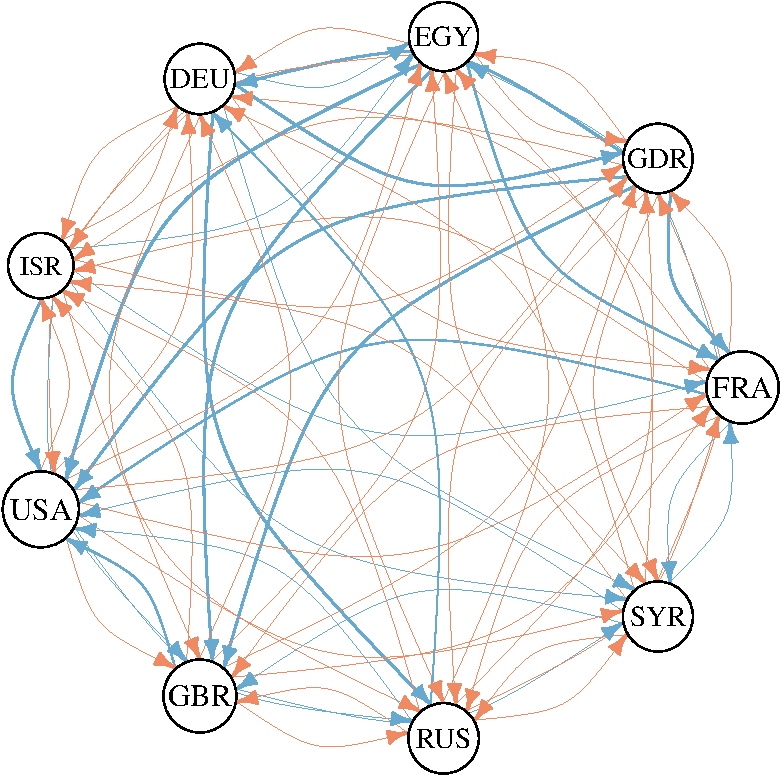
\includegraphics[width=.5\textwidth]{compNet_1972}
%		\label{fig:comp72}} & 
%
%	\subfloat[sub1][Compliance: 1992]{
%		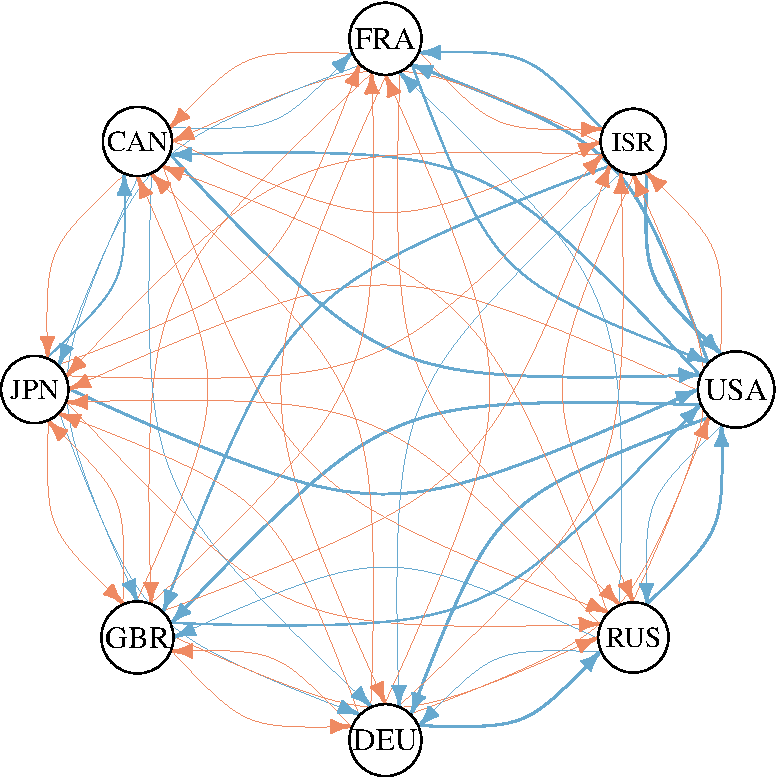
\includegraphics[width=.5\textwidth]{compNet_1992}
%		\label{fig:comp92}} \\
%
%	\multicolumn{2}{c}{\subfloat[sub1][Compliance: 2012]{
%			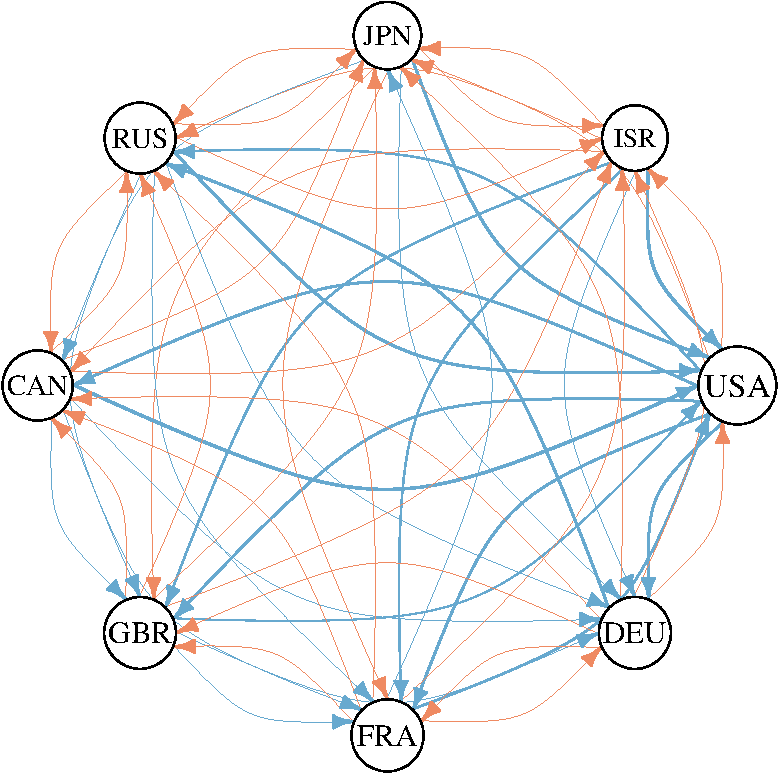
\includegraphics[width=.5\textwidth]{compNet_2012}
%			\label{fig:comp02}}}
%
%	% \subfloat[sub1][Sanction: 1972]{
%	% 	\includegraphics[width=.33\textwidth]{sancNet_1972}
%	% 	\label{fig:sanc72}} & 
%
%	% \subfloat[sub1][Sanction: 1992]{
%	% 	\includegraphics[width=.33\textwidth]{sancNet_1992}
%	% 	\label{fig:sanc92}} & 
%
%	% \subfloat[sub1][Sanction: 2012]{
%	% 	\includegraphics[width=.33\textwidth]{sancNet_2012}
%	% 	\label{fig:sanc02}}
%
%	\end{tabular}
%	\label{fig:recipNet}
%\end{figure}
%\FloatBarrier

